\documentclass[10,portrait]{article}
\usepackage{lmodern}
\usepackage{amssymb,amsmath}
\usepackage{ifxetex,ifluatex}
\usepackage{fixltx2e} % provides \textsubscript
\ifnum 0\ifxetex 1\fi\ifluatex 1\fi=0 % if pdftex
  \usepackage[T1]{fontenc}
  \usepackage[utf8]{inputenc}
\else % if luatex or xelatex
  \ifxetex
    \usepackage{mathspec}
  \else
    \usepackage{fontspec}
  \fi
  \defaultfontfeatures{Ligatures=TeX,Scale=MatchLowercase}
\fi
% use upquote if available, for straight quotes in verbatim environments
\IfFileExists{upquote.sty}{\usepackage{upquote}}{}
% use microtype if available
\IfFileExists{microtype.sty}{%
\usepackage[]{microtype}
\UseMicrotypeSet[protrusion]{basicmath} % disable protrusion for tt fonts
}{}
\PassOptionsToPackage{hyphens}{url} % url is loaded by hyperref
\usepackage[unicode=true]{hyperref}
\PassOptionsToPackage{usenames,dvipsnames}{color} % color is loaded by hyperref
\hypersetup{
            pdftitle={Meeting minutes from the Biology Postdoc Cohort at Emory},
            colorlinks=true,
            linkcolor=blue,
            citecolor=red,
            urlcolor=blue,
            breaklinks=true}
\urlstyle{same}  % don't use monospace font for urls
\usepackage[margin=1in]{geometry}
\usepackage[]{biblatex}
\usepackage{graphicx,grffile}
\makeatletter
\def\maxwidth{\ifdim\Gin@nat@width>\linewidth\linewidth\else\Gin@nat@width\fi}
\def\maxheight{\ifdim\Gin@nat@height>\textheight\textheight\else\Gin@nat@height\fi}
\makeatother
% Scale images if necessary, so that they will not overflow the page
% margins by default, and it is still possible to overwrite the defaults
% using explicit options in \includegraphics[width, height, ...]{}
\setkeys{Gin}{width=\maxwidth,height=\maxheight,keepaspectratio}
\IfFileExists{parskip.sty}{%
\usepackage{parskip}
}{% else
\setlength{\parindent}{0pt}
\setlength{\parskip}{6pt plus 2pt minus 1pt}
}
\setlength{\emergencystretch}{3em}  % prevent overfull lines
\providecommand{\tightlist}{%
  \setlength{\itemsep}{0pt}\setlength{\parskip}{0pt}}
\setcounter{secnumdepth}{0}
% Redefines (sub)paragraphs to behave more like sections
\ifx\paragraph\undefined\else
\let\oldparagraph\paragraph
\renewcommand{\paragraph}[1]{\oldparagraph{#1}\mbox{}}
\fi
\ifx\subparagraph\undefined\else
\let\oldsubparagraph\subparagraph
\renewcommand{\subparagraph}[1]{\oldsubparagraph{#1}\mbox{}}
\fi

% set default figure placement to htbp
\makeatletter
\def\fps@figure{htbp}
\makeatother


\title{Meeting minutes from the Biology Postdoc Cohort at Emory}
\author{Matthew Malishev\textsuperscript{1}* \& Molly
Gallagher\textsuperscript{1}\\[2\baselineskip]\emph{\textsuperscript{1}
Department of Biology, Emory University, 1510 Clifton Road NE, Atlanta,
GA, USA, 30322}}
\date{}

\begin{document}
\maketitle

{
\hypersetup{linkcolor=black}
\setcounter{tocdepth}{2}
\tableofcontents
}
\newpage   

Date: 2019-01-11\\
R version: 3.5.0\\
*Corresponding author:
\href{mailto:matthew.malishev@emory.edu}{\nolinkurl{matthew.malishev@emory.edu}}\\
This document can be found at
\url{https://github.com/darwinanddavis/emory_postdocs}

~

Session info

\begin{verbatim}
R version 3.5.0 (2018-04-23)
Platform: x86_64-apple-darwin15.6.0 (64-bit)
Running under: OS X El Capitan 10.11.6

Matrix products: default
BLAS: /Library/Frameworks/R.framework/Versions/3.5/Resources/lib/libRblas.0.dylib
LAPACK: /Library/Frameworks/R.framework/Versions/3.5/Resources/lib/libRlapack.dylib

locale:
[1] en_US.UTF-8/en_US.UTF-8/en_US.UTF-8/C/en_US.UTF-8/en_US.UTF-8

attached base packages:
[1] stats     graphics  grDevices utils     datasets  methods   base     

loaded via a namespace (and not attached):
 [1] compiler_3.5.0  backports_1.1.2 magrittr_1.5    rprojroot_1.3-2 tools_3.5.0     htmltools_0.3.6
 [7] pillar_1.2.3    tibble_1.4.2    yaml_2.2.0      Rcpp_0.12.19    stringi_1.2.3   rmarkdown_1.10 
[13] knitr_1.20      stringr_1.3.1   digest_0.6.15   rlang_0.3.0.1   evaluate_0.10.1
\end{verbatim}

\newpage  

\subsection{Overview}\label{overview}

This document contains the meeting minutes from the Biology Postdoc
Cohort at Emory.

The group hosts regular meetups to learn about what the postdocs in
Biology at Emory are doing, harness cool research skills and tools that
everyone uses, foster research overlaps, brainstorm and troubleshoot
ideas, discuss weird results that nobody knows the answer to, practise
upcoming seminars, and simply build a stronger postdoc culture in
Biology at Emory.

Questions and suggestions welcome at
\href{mailto:matthew.malishev@emory.edu}{\nolinkurl{matthew.malishev@emory.edu}}.

\newpage  

\subsection{TO DO list}\label{to-do-list}

\begin{itemize}
\tightlist
\item
  Add attending postdocs to OPE Emory list (Beverly)\\
\item
  Come up with a cooler name for the group\\
\item
  Other things\\
\item
  Aim for a collaborative paper
\end{itemize}

\subsubsection{\texorpdfstring{\emph{Next meetup:} February 8,
2019}{Next meetup: February 8, 2019}}\label{next-meetup-february-8-2019}

\newpage  

\subsection{February 8, 2019}\label{february-8-2019}

\newpage  

\subsection{January 11, 2019}\label{january-11-2019}

IMPACT statement workshop

\href{https://xkcd.com/}{XKCD} inspired page for communicating your
ideas using just the ten hundred most commonly-used words:
\href{http://splasho.com/upgoer5/}{The Up-Goer Five Text Editor}

\begin{figure}
\centering
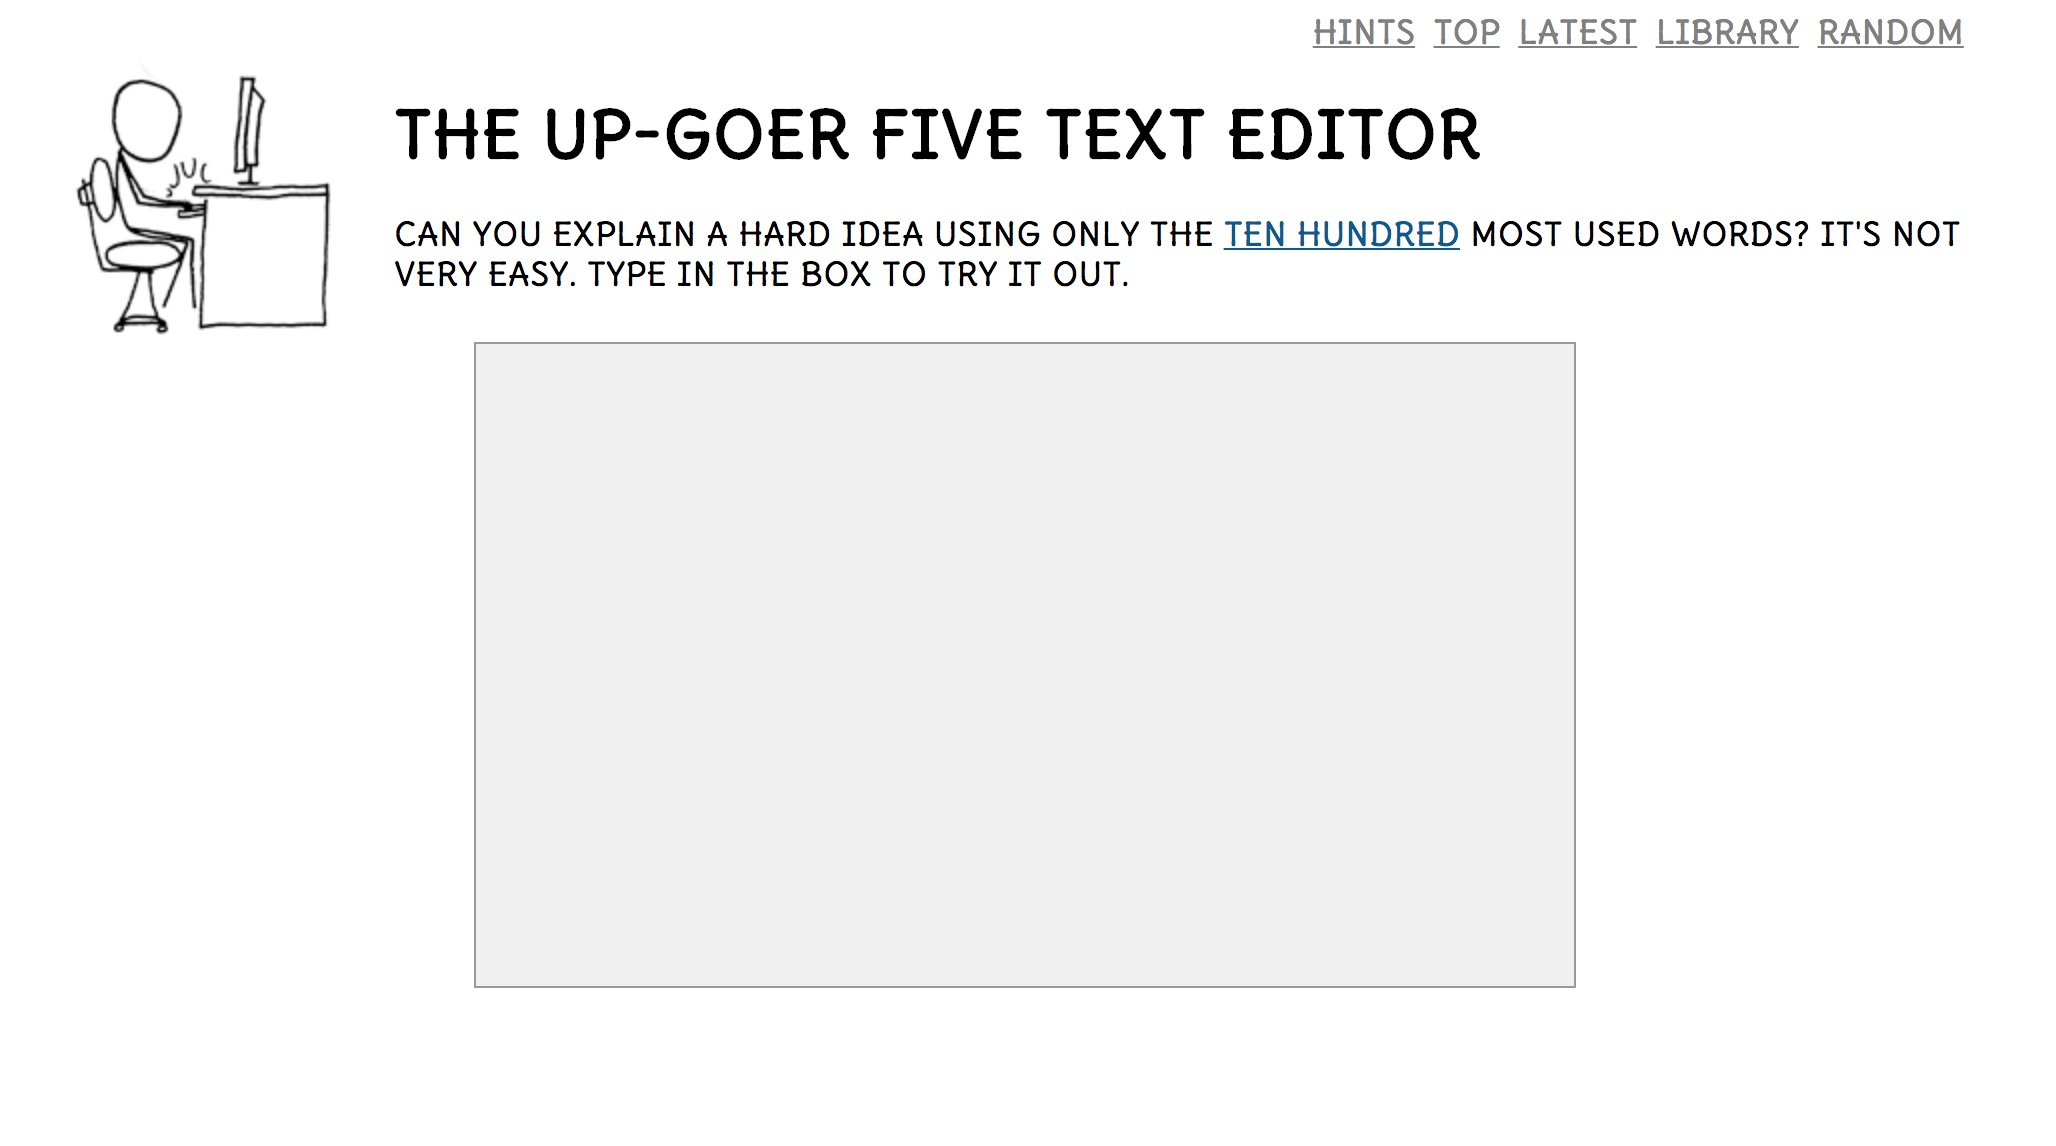
\includegraphics{upgoer5.jpeg}
\caption{Check out this page for practical ways of communicating your
super complex research: \href{http://splasho.com/upgoer5/}{The Up-Goer
Five Text Editor}}
\end{figure}

\subsubsection{Some writing guides from the
masses}\label{some-writing-guides-from-the-masses}

\href{https://www.amazon.com/Elements-Style-William-Strunk-Jr/dp/194564401X}{The
Elements of Style by Strunk and White}

\href{http://people.vetmed.wsu.edu/jmgay/courses/documents/TheParamedicMethod.pdf}{Revising
Prose by Richard Lanham}

\href{https://www.amazon.com/Ideas-into-Words-Mastering-Science/dp/0801873304/ref=pd_sim_b_1}{Idead
into Words by Elise Hancock} \textbf{Matt's personal favourite}

\newpage    

\subsection{December 14, 2018}\label{december-14-2018}

\subsection{\texorpdfstring{\emph{Biosketch of
postdocs}}{Biosketch of postdocs}}\label{biosketch-of-postdocs}

\textbf{Matt Malishev}\\
Civitello lab\\
Bioenergetics and individual-based modelling of host-parasite dynamics
of human schistosome populations; spatial simulation modelling;
metabolic theory

\textbf{Molly Gallagher}\\
Koelle lab\\
Disease ecology; differential equation models; current work focuses on
modeling defective interfering particles in influenza

\textbf{Aileen Berasategui Lopez}\\
Gerardo lab\\
The genomic and chemical basis of host-fidelity

\textbf{Caitlin Conn}\\
Gerardo lab\\
Host range and its genetic basis in a mycoparasite

\textbf{Jeremy Harris}\\
Koelle lab\\
Current IAV modeling: Passage study modeling, estimating bottleneck
sizes

\textbf{Mary Bushman}\\
Rustom lab\\
Linking within- and between-host dynamics of infectious diseases
(modeling)

\textbf{David Nicholson}\\
Prinz lab\\
``Lifelong Learning Machines'' -- continual machine learning algorithms

\textbf{Julien Catanese}\\
Jaeger lab

\textbf{Derrick Morton}\\
Corbett lab\\
Studying how defects in RNA processing lead to neurodegenerative
disesase

\textbf{Scott Villa}\\
Gerardo lab\\
Role of endysymbionts in driving host reproductive isolation and
adaptive radiation

\textbf{Rohan Mehta}\\
Weissman Lab\\
Evolution in spatially-structured populations

\subsubsection{Workshop ideas}\label{workshop-ideas}

IMPACT workshop\\
- Impact of science + advancement in research\\
Contact: Derrick

\newpage  

\subsection{November 30, 2018}\label{november-30-2018}

\subsubsection{Outcomes for postdoc
group}\label{outcomes-for-postdoc-group}

Meetings every second and fourth week

Talk therapy among working class postdocs

Intro talks from postdocs to group

\begin{itemize}
\item
  Lightning, 2-min talk for group
\item
  New postdocs give a brief intro talk for their first meeting
\end{itemize}

Postdoc mentorship group for assisting grad students during qualifying
exams

\begin{itemize}
\item
  Online directory of postdocs showcasing background and expertise.
  Include non-science background stuff, such as applying for
  international universities.\\
  The journal peer review system and open access science
\item
  Using \emph{bioarXiv} and pre-prints\\
\item
  Open access science\\
\item
  Writing a paper on the science peer review system from postdoc
  perspective
\end{itemize}

\newpage  

\subsection{November 1, 2018}\label{november-1-2018}

\paragraph{Ideas for things people
want}\label{ideas-for-things-people-want}

Collaborate on overlapping research\\
Brainstorm ideas\\
Present new results\\
Practise conference talks\\
Writing retreats\\
Regular coding/math club

\paragraph{Bigger ideas}\label{bigger-ideas}

Combine other labs/departments\\
- other biology floor levels\\
- math/env sciences

\newpage  

\subsection{Links and ideas}\label{links-and-ideas}

\printbibliography

\end{document}
